\documentclass[dvipdfmx,cjk]{beamer} 
\usepackage{graphicx}
\usepackage{tikz}
\usetheme{CambridgeUS} 

\AtBeginSection{\frame{\sectionpage}}
\AtBeginSubsection{\frame{\subsectionpage}}
\AtBeginSubsubsection{\frame{\subsubsectionpage}}

\begin{document}


\title[Halide]{ステンシル計算言語Halide}
\author[T. Muranushi]{村主崇行\\special thanks: 似鳥啓吾}            %% ここに書かれた情報は色々なところに使われるので
\institute[RIKEN/AICS]{計算科学研究機構}   %% なるべく設定した方が良い

\begin{frame}                  %% \begin{frame}..\end{frame} で 1 枚のスライド
\titlepage                     %% タイトルページ
\end{frame}

\begin{frame}                  %% 目次 (必要なければ省略)
\tableofcontents
\end{frame}

\section{はじめに} 

\begin{frame}\frametitle{ステンシル計算とは?}
配列変数を更新していくタイプのアルゴリズムで、配列の各要素を、それぞれ近傍の要素の値のみに基づき、同じルールで更新
するものをいう。

\pause

要するに

\pause

配列ベースの流体計算、MHD、等々
\end{frame}

\begin{frame}\frametitle{Halideとは?}
Halideはステンシル計算プログラムの生成とチューニングのためのライブラリ。
画像処理のために開発された。\cite{ragan2012decoupling,ragan2013halide}


\begin{center}
  \begin{tabular}{|c|c|c|}
    \hline
    &Paraiso & Halide\\
    \hline
    基本言語 & Haskell & C++ \\
    コード生成対象 & x86, CUDA &
    \multicolumn{1}{p{5cm}|}{x86/SSE, ARM, Native Client, OpenCL, CUDA,  ... }\\
    扱える次元 & n次元 & n次元 \\ 
    最適化の種類 & ループ融合、同期 & \multicolumn{1}{p{5cm}|}{並列度、局所性、計算節約 の間のトレードオフ} \\ 
    自動チューニング & あり & なし \\ 
    \hline
  \end{tabular}
\end{center}
\end{frame}

\section{Halideの文法} 
\begin{frame}[fragile]\frametitle{Halideの文法}

プログラミング言語Halideは、 C++のライブラリとして実装されている。

したがってHalideでプログラムするということはC++のプログラムを書くことになる。

基本的な型として、$n$次元配列を表す{\tt Func}と、配列添字変数を表す{\tt Var}
があり、これらを組み合わせてステンシル計算を記述する。

\pause

\begingroup
    \fontsize{8pt}{9pt}\selectfont
\begin{verbatim}
Func input = initial_condition.realize(NX,NY);
Var i,j;
Func cell2 = (input(i-1,j)+input(i,j)+input(i+1,j))/3;
Func output = (input(i,j-1)+input(i,j)+input(i,j+1))/3;
\end{verbatim}
\endgroup

\pause

以上のような構文を実現するため、C++の演算子オーバーロードを多用している。
例えば、複数引数関数のように見えるものは括弧演算子
{\tt operator()}をオーバーロードすることで
実現している。

\end{frame}


\begin{frame}[fragile]\frametitle{Halideのプログラムの例}

Halideではステンシル計算をとても直感的な形で記述することができる。

\pause

たとえば、以下のような拡散方程式の離散化解法は
\begin{eqnarray}
C_\mathrm{in} &=& \mathrm{initial~condition} \\
C_2 [i,j] &=& \frac{1}{3}\left(C_\mathrm{in}[i-1,j] + C_\mathrm{in}[i,j] + C_\mathrm{in}[i+1,j]\right) \\
C_\mathrm{out} [i,j] &=& \frac{1}{3}\left(C_\mathrm{2}[i,j-1] + C_\mathrm{2}[i,j] + C_\mathrm{2}[i,j+1]\right)
\end{eqnarray}

\pause

Halideではこのように記述できる。
\begin{center}
\begingroup
    \fontsize{9pt}{10pt}\selectfont
\begin{verbatim}
    Var i,j;
    Func input = initial_condition.realize(NX,NY);
    Func cell2 = (input(i-1,j)+input(i,j)+input(i+1,j))/3;
    Func output = (input(i,j-1)+input(i,j)+input(i,j+1))/3;
\end{verbatim}
\endgroup
\end{center}

\end{frame}


\begin{frame}[fragile]\frametitle{Halideのコード生成と実行}

Halideで配列変数としてもっとも頻繁に登場する
{\tt Func}型は、「その配列を計算するための手続き」を保持しているにすぎない。
これに対し{\tt Image}型は実際にメモリ上に確保された多次元配列である。

{\tt realize()}関数を呼び出して
{\tt Func}型を
{\tt Image}型に変換したとき、コード生成・最適化・実際の計算が行われる。
(プログラムに変更がなければ、いったん生成されたコードは使いまわされる)

\begingroup
    \fontsize{9pt}{10pt}\selectfont
\begin{verbatim}
    inPar.set(input);
    output=cell3.realize(NX,NY);
\end{verbatim}
\endgroup

\end{frame}

\begin{frame}[fragile]\frametitle{Halideにおけるステンシル計算の実装}
\begin{itemize}
\item {\tt Image}:実際にメモリ上に確保された配列
\item {\tt Func}:配列を操作するプログラムを構成するデータフローグラフの要素
\item {\tt ImageParam}:{\tt Image}へのポインタ、データフローグラフの入力点
\end{itemize}

xxx: DFGの絵

\end{frame}



\begin{frame}[fragile]\frametitle{Halideにおけるステンシル計算の実装例}

\begingroup
    \fontsize{9pt}{10pt}\selectfont
\begin{verbatim}
  Var x,y;             // 配列添字を表す変数
  Image input, output; // 計算結果を格納する配列変数
  ImageParam inPar;    // Halideプログラムの入力
  Func cell2 = a * inPar(x,y) + b * inPar(x+1,y); // Halideプログラム
  Func cell3 = c * cell2(x,y) + d * cell2(x,y+1); // Halideプログラム

  // 計算戦略を指定
  cell3.split(y, yo, yi, 16).parallel(yo).parallel(yo).vectorize(x,4);
  cell2.store_at(cell3,yo).compute_at(cell3,yi).vectorize(x,4);

  for (int t=0; t<=MAX_T; ++t) {
    inPar.set(input);             // プログラムに入力を設定
    output=cell3.realize(NX,NY);  // プログラムを実行
    std::swap(input, output);     // 出力を次のタイムステップの入力へ交換
  }


\end{verbatim}
\endgroup


\end{frame}


\begin{frame}[fragile]\frametitle{Halideのコード生成}

生成されたコードはその場で主プログラムにリンクされて実行される(Just in Time compile, JIT)
のほか、C++言語ソースやアセンブリ、LLVMバイトコードをファイルに生成させ、のちほど利用する(Ahead of Time compile, AOT)こともできる。

\begingroup
    \fontsize{9pt}{10pt}\selectfont
\begin{verbatim}
        compile_to_assembly
        compile_to_bitcode
        compile_to_c
        compile_to_file
        compile_to_function_pointers
        compile_to_header
        compile_to_lowered_stmt
        compile_to_native
        compile_to_object
        compile_to_src
\end{verbatim}
\endgroup

\end{frame}


\begin{frame}[fragile]\frametitle{コデザイン用コード生成言語としてのHalide/LLVM}

例えば、Halideから{\tt .bc}ファイルを生成した上で、Bulldozer向けアセンブリを生成させることで、
fma(融合加乗算)命令を含むアセンブリを生成できる。

\begingroup
    \fontsize{8pt}{9pt}\selectfont
\begin{verbatim}
$ clang -O1 -march=bdver1 -ffp-contract=fast blur.bc -S
$ less blur.s
...
	vfmaddss	%xmm3, (%r11,%rdi,4), %xmm1, %xmm3
	vfmaddss	%xmm3, (%r11,%r10,4), %xmm1, %xmm3
	vfmaddss	%xmm4, (%r11,%rax,4), %xmm1, %xmm4
	vfmaddss	%xmm4, (%r11,%r14,4), %xmm1, %xmm4
	vmulss	%xmm0, %xmm4, %xmm4
...
\end{verbatim}
\endgroup

これはGrape-Xのようなfmaをサポートするハードウェア向けのコード生成にも流用できると思われる。


\end{frame}


\section{Halideの最適化} 
\begin{frame}\frametitle{Halideの最適化空間}

Halideは、ステンシル計算の最適化問題を、
低並列度、演算重複、メモリ負荷、の間のトレードオフがある中で
計算とメモリの粒度を操作することで、計算の速度を最大化する
問題と捉えている。

計算とメモリの粒度とは何か?以下、拡散方程式を例に見ていく。

\begin{center}
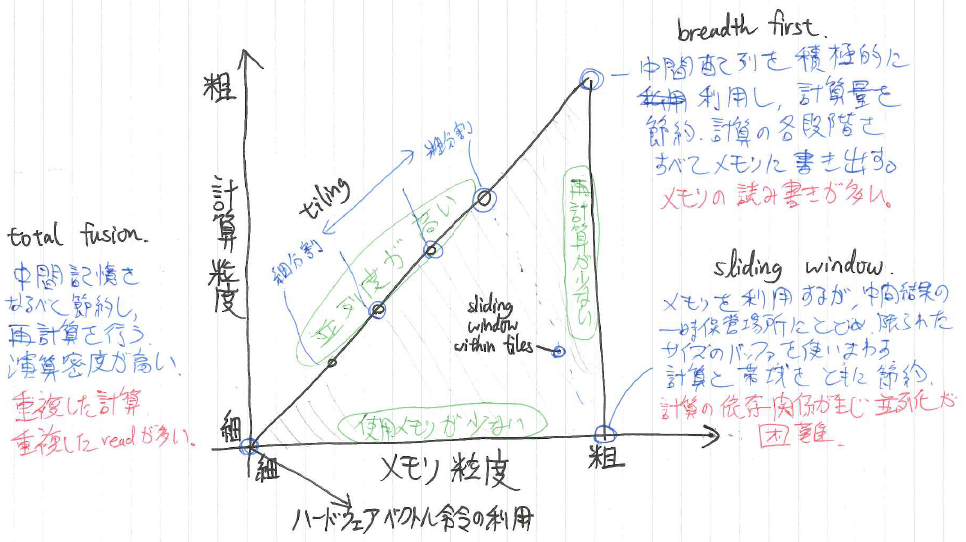
\includegraphics[width=8cm]{figure/doc/schedule-space.png}
\end{center}
\end{frame}


\begin{frame}\frametitle{Halideの最適化空間:粗メモリ、粗計算}

\begingroup \footnotesize
\begin{eqnarray*}
C_\mathrm{in} &=& \mathrm{initial~condition} \\
C_\mathrm{blurx} [i,j] &=& \frac{1}{3}\left(C_\mathrm{in}[i-1,j] + C_\mathrm{in}[i,j] + C_\mathrm{in}[i+1,j]\right) \\
C_\mathrm{out} [i,j] &=& \frac{1}{3}\left(C_\mathrm{2}[i,j-1] + C_\mathrm{2}[i,j] + C_\mathrm{2}[i,j+1]\right)
\end{eqnarray*}
\endgroup


\begin{center}
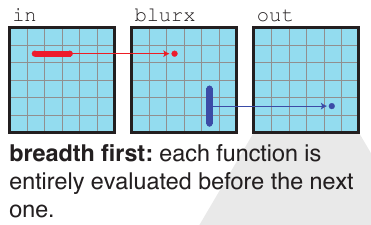
\includegraphics[width=4cm]{figure/doc/blur-breadth-first.png}
\end{center}


$C_\mathrm{blurx} [i,j]$ を全て計算し、メモリに置いてから、それを利用して
$C_\mathrm{out} [i,j]$を計算する。



\end{frame}


\begin{frame}\frametitle{Halideの最適化空間:細メモリ、細計算}

\begingroup \footnotesize
\begin{eqnarray*}
C_\mathrm{in} &=& \mathrm{initial~condition} \\
C_\mathrm{blurx} [i,j] &=& \frac{1}{3}\left(C_\mathrm{in}[i-1,j] + C_\mathrm{in}[i,j] + C_\mathrm{in}[i+1,j]\right) \\
C_\mathrm{out} [i,j] &=& \frac{1}{3}\left(C_\mathrm{2}[i,j-1] + C_\mathrm{2}[i,j] + C_\mathrm{2}[i,j+1]\right)
\end{eqnarray*}
\endgroup


\begin{center}
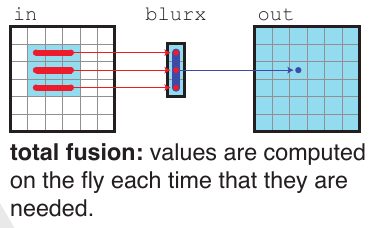
\includegraphics[width=4cm]{figure/doc/blur-fusion.png}
\end{center}

中間記憶を最低限しか使わず、$C_\mathrm{out} [i,j]$の各要素を計算するたびに、必要な$C_\mathrm{blurx} [i,j]$ の要素を全て再計算する。


\end{frame}

\begin{frame}\frametitle{Halideの最適化空間:粗メモリ、細計算}

% \begingroup \footnotesize
% \begin{eqnarray*}
% C_\mathrm{in} &=& \mathrm{initial~condition} \\
% C_\mathrm{blurx} [i,j] &=& \frac{1}{3}\left(C_\mathrm{in}[i-1,j] + C_\mathrm{in}[i,j] + C_\mathrm{in}[i+1,j]\right) \\
% C_\mathrm{out} [i,j] &=& \frac{1}{3}\left(C_\mathrm{2}[i,j-1] + C_\mathrm{2}[i,j] + C_\mathrm{2}[i,j+1]\right)
% \end{eqnarray*}
% \endgroup


\begin{center}
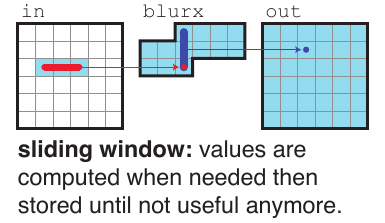
\includegraphics[width=4cm]{figure/doc/blur-sliding-window.png}
\end{center}

$C_\mathrm{out} [i,j]$の各要素を計算するたびに、新たな
$C_\mathrm{blurx} [i,j]$ の要素を計算するが、それを保持しておき再利用。
これ以上利用されなくなった時に破棄。中間結果をぴったり保持できるだけのバッファ
(この例だと3行分)を使いまわす。


\end{frame}


\begin{frame}\frametitle{粗メモリ粗計算と細メモリ細計算の中間}


\begin{center}
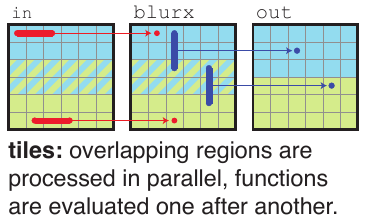
\includegraphics[width=4cm]{figure/doc/blur-tiles.png}
\end{center}

配列を1次元または2次元のタイルに分割し、タイル1個分を記憶できるだけのバッファを用意し、
その中ではすべての中間結果を保持する。タイルバッファを使いまわす。

タイルバッファのサイズがキャッシュに収まるときには高性能が期待できる。

\end{frame}

\begin{frame}\frametitle{すべての中間}


\begin{center}
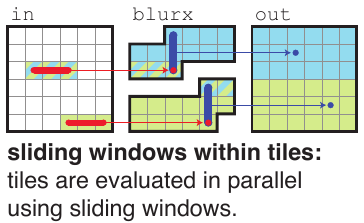
\includegraphics[width=4cm]{figure/doc/blur-sliding-within-tiles.png}
\end{center}

配列を1次元または2次元のタイルに分割し、タイル1個分を記憶できるだけのバッファを用意し、
その中では最低限のの中間結果を保持するバッファを使いまわす。
タイルごとの計算は並列に行う。



\end{frame}


\begin{frame}\frametitle{Halideの最適化空間}

\begin{center}
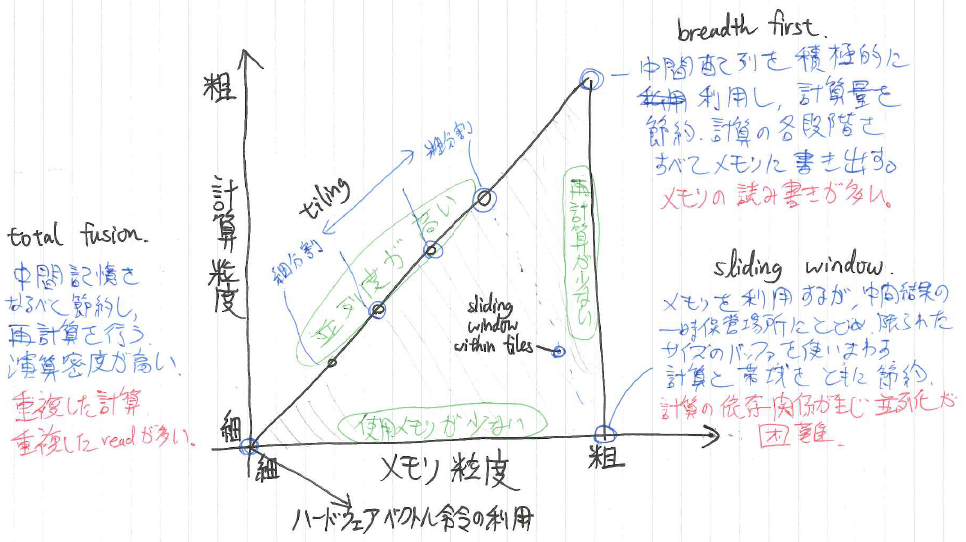
\includegraphics[width=12cm]{figure/doc/schedule-space.png}
\end{center}
\end{frame}



\begin{frame}\frametitle{Halideがサポートするプログラム変換の種類}

ステンシル計算の実装空間を探求するため、Halideはさまざまなプログラム変換をサポートする。

\begin{itemize}
  \item 分割:1..(M*N)までのループを1..Mと1..Nの二重ループに分割する
  \item 融合:1..Mと1..Nの2つのループを1つにまとめてしまう
  \item スレッド並列化:各添字を並列に計算
  \item アンロール:固定長のループを全部展開してループを消す
  \item ベクトル化:固定長のループをベクトル命令に置き換える
  \item タイル化:2次元のブロックを用意しそれを更新
  \item 入れ子ループの入れ替え
  \item 特殊化:条件変数が真の場合と偽の場合でループを分けループの中身を簡単化
\end{itemize}
\end{frame}

\begin{frame}\frametitle{プログラム変換:ループ分割}
\begin{center}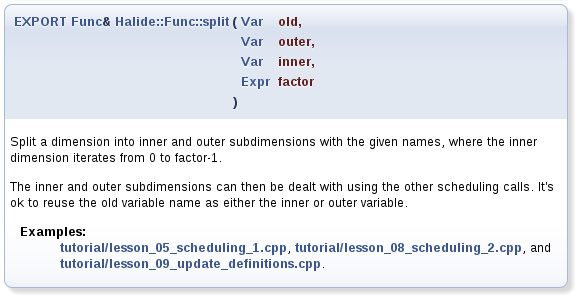
\includegraphics[width=11cm]{figure/doc/schedule-split.png}\end{center}\end{frame}

\begin{frame}\frametitle{プログラム変換:ループ融合}
\begin{center}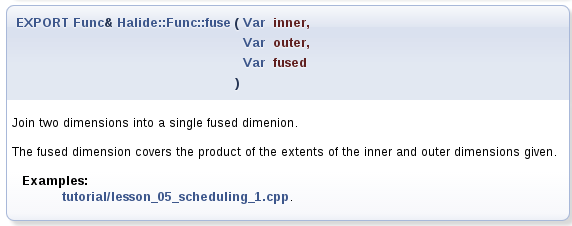
\includegraphics[width=11cm]{figure/doc/schedule-fuse.png}\end{center}\end{frame}

\begin{frame}\frametitle{プログラム変換:並列化}
\begin{center}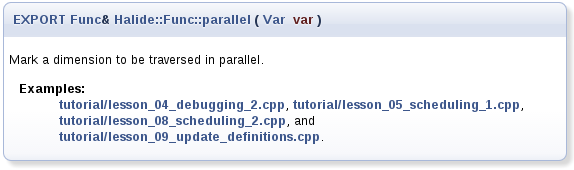
\includegraphics[width=11cm]{figure/doc/schedule-parallel.png}\end{center}\end{frame}

\begin{frame}\frametitle{プログラム変換:アンロール}
\begin{center}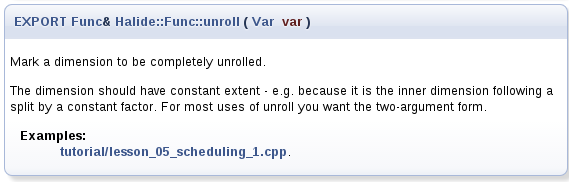
\includegraphics[width=11cm]{figure/doc/schedule-unroll.png}

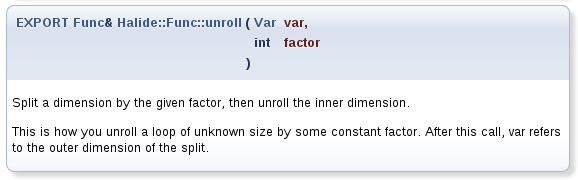
\includegraphics[width=11cm]{figure/doc/schedule-unroll2.png}
\end{center}\end{frame}

\begin{frame}\frametitle{プログラム変換:ベクトル化}
\begin{center}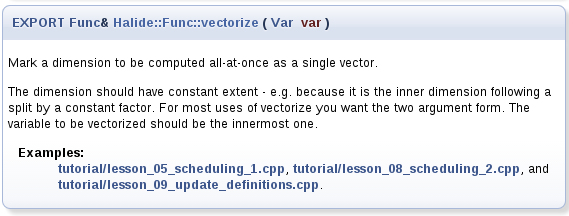
\includegraphics[width=11cm]{figure/doc/schedule-vectorize.png}

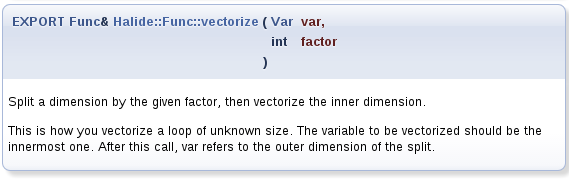
\includegraphics[width=11cm]{figure/doc/schedule-vectorize2.png}
\end{center}\end{frame}

\begin{frame}\frametitle{プログラム変換:タイル分割}
\begin{center}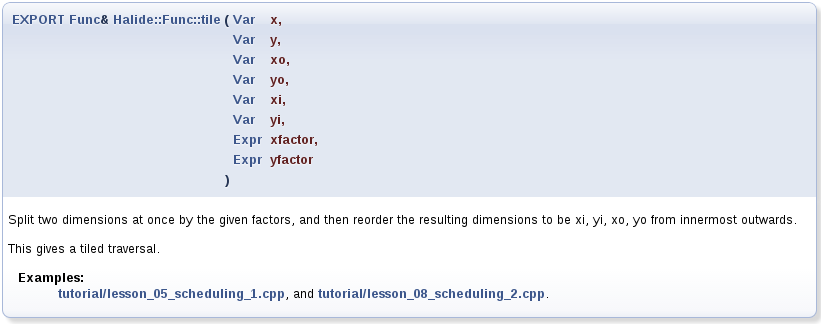
\includegraphics[width=11cm]{figure/doc/schedule-tile.png}\end{center}\end{frame}



\section{ベンチマーク実験}
\begin{frame}\frametitle{ベンチマーク対象と環境}

以下のようなマシンで、拡散程式ソルバをスケジュールや問題サイズを変えて実行し、性能の変化を調べた。
似鳥さん、マシンを用意してくれてありがとう!

\begin{center}
  \begin{tabular}{|c|c|}
    \hline
    マシン名 & armagnac0\\
    CPU & Bulldozer, 64 cores \\
    Memory & 256GB \\
    \hline
  \end{tabular}
\end{center}

\begin{itemize}
\item ノートPCだと一晩かかったLLVMのビルドが数分
\item {\tt llvm\$ make -j } fork爆弾事件
\end{itemize}
\end{frame}


\begin{frame}[allowframebreaks]{参考文献}{}
  \bibliographystyle{apalike}
  \bibliography{bunken}
\end{frame}



% \begin{bibliography}
% 
% \bibitem[de~Saussure, 1995]{Saussure1995}
% de~Saussure, F. (1995).
% \newblock {\em Cours de Linguistique Grale}.
% \newblock Payot.
% 
% \bibitem[Labov, 1972]{Labov1972}
% Labov, W. (1972).
% \newblock {\em Sociolinguistic Patterns}.
% \newblock University of Pennsylvania Press, Philadelphia.
% 
% \end{bibliography}








\section*{リサイクルボックス}




\subsection{}
\begin{frame}\frametitle{}
\begin{eqnarray}
\end{eqnarray}
\end{frame}


\begin{frame}[fragile]\frametitle{}
\begingroup
    \fontsize{8pt}{9pt}\selectfont
\begin{verbatim}
subroutine kernel__velderiv()
\end{verbatim}
\endgroup
\vspace{-1cm}
\end{frame}




\end{document}

